\chapter{Chapter 6: Filesystems}\label{ch-filesystems}

\section{Introduction}\label{introduction}

Given that both the processor and the main memory are resources in the
system, till this point, we have seen how a kernel of an operating
system works as a resource manager, 539kernel manages these resources
\footnote{Incompletely of course, to keep 539kernel as simple as
  possible, only the basic parts of resources management were presented.}
and provides them to the different processes in the system.

Another role of a kernel is to provide a way to communicate with
external devices, such as the keyboard and hard disk. \emph{Device
drivers} are the way of realizing this role of the kernel. The details
of the external devices and how to communicate with them are low-level
and may be changed at any time. The goal of a device driver is to
communicate with a given device by using the device's own
language\footnote{The word \emph{language} here is a metaphor, it
  doesn't mean a programming language.} in behalf of any component of
the system (e.g.~a process) that would like to use the device. Device
drivers provide an interface so it can be called by the other system's
components in order to tell the device something to do, we can consider
this interface as a library that we use in normal software development.
In this way, the low-level details of the device is hidden from the
other components and whenever these details changed only the code of the
device driver should be changed, the interface can be kept to not affect
its users. Also, hiding the low-level details from driver's user can
ensure the simplicity of using that driver.

The matter of hiding the low-level details with something higher-level
is too important and can be found, basically, everywhere in computing
and the kernels are not an exception of that. Of course, there is
virtually no limit of providing higher-level concepts based on a
previous lower-level concept, also, upon something that we consider as a
high-level concept we can build something even higher-level. Beside the
previous example of device drivers, one of obvious examples where the
kernels fulfill the role of hiding the low-level details and providing
something higher-level, in other words, providing an \emph{abstraction},
is a filesystem which provides the well-known abstraction, a file.

In this chapter we are going to cover these two topics, device drivers
and filesystem by using 539kernel. As you may recall, it turned out that
accessing to the hard disk is an important aspect for virtual memory,
so, to be able to implement virtual memory, the kernel itself needs to
access the hard disk which makes it an important component in the
kernel, so, we are going to implement a device driver that communicate
with the hard disk in this chapter. After getting the ability of reading
from the hard disk or writing to it, we can explore the idea of
providing abstractions by the kernel through writing a filesystem that
uses the hard disk device driver and provides a higher-level view of the
hard disk that we all familiar with instead of the physical view of the
hard disk which has been described previously in chapter
\ref{ch-bootloader}. The final result of this chapter is version
\lstinline!NE! of 539kernel.

\section{ATA Device Driver}\label{ata-device-driver}

No need to say the hard disks are too common devices that are used as
secondary storage devices. There are a lot of manufacturers that
manufacture hard disks and sell them, imagine for a moment that each
hard disk from a different manufacturer use its own way for the
communication between the software and the hard disk, that is, the
method \lstinline!X! should be used to be able to communicate with hard
disks from manufacturer \lstinline!A! while the method \lstinline!Y!
should be used with hard disks from manufacturer \lstinline!B! and so
on, given that there are too many manufacturers, this will be a
nightmare. Each hard disk will need its own device driver which talks a
different language from the other hard disk device drivers.

Fortunately, this is not the case, at least for the hard disks, in these
situations, standards are here to the rescue. A manufacturer may design
the hard disk hardware in anyway, but when it comes to the part of the
communication between the hard disk and the outside world, a standard
can be used, so, any device driver that works with this given standard
will be able to communicate with this new hard disk. There are many
well-known standards that are related to the hard disks, \emph{small
computer system interface} (SCSI) is one of them, another one is
\emph{advanced technology attachment} (ATA), another well-known name for
ATA is \emph{Integrated Drive Electronics} (IDE). The older ATA standard
is now known as Parallel ATA (PATA) while the newer version of ATA is
known as Serial ATA (SATA). Because ATA is more common in personal
computers we are going to focus on it here and write a device driver for
it, SCSI is more common in servers.

As in PIC which has been discussed in chapter \ref{ch-progenitor}, ATA
hard disks can be communicated with by using port-mapped I/O
communication through the instructions \lstinline!in! and
\lstinline!out!. But before discussing the ATA commands that let us to
issue a read or write request to the hard disk, let's write two routines
in assembly that can be used used as C functions in C code and perform
the same functionality of the instructions \lstinline!in! and
\lstinline!out!.

If you don't recall, the instruction \lstinline!out! is used to write
some bytes on a given port number, so, if we know the port number that a
device (e.g.~hard disk) receives commands from, we can use the
instruction \lstinline!out! to write a valid command to that port. On
the other hand, the instruction \lstinline!in! reads data from a given
port, for example, sometimes after we send a command to a device, it
responds by writing something on a specific port, the instruction
\lstinline!in! can be used to read this value.

The assembly code of the both routines that we are going to define next
should reside in \lstinline!starter.asm! anywhere between
\lstinline!bits 32! and the beginning of \lstinline!start_kernel!
routine. The following is the code of \lstinline!dev_write! which can be
used by C kernel code to write to a given port. In C, we can see that it
has this prototype: \lstinline!dev_write( int port, int cmd )!.

\begin{lstlisting}
dev_write:
    ; Part 1
    push edx
    push eax
    
    ; Part 2
    xor edx, edx
    xor eax, eax
    
    ; Part 3
    mov dx, [esp + 12]
    mov al, [esp + 16]
    
    ; Part 4
    out dx, al 
    
    ; Part 5
    pop eax
    pop edx
    
    ret
\end{lstlisting}

The core part of this routine is part four which contains the
instruction \lstinline!out! that sends the value of \lstinline!AL! to
the port number which is stored in \lstinline!DX!. Because we are using
these two registers \footnote{Which are, as you know, parts of the
  registers \lstinline!EAX! and \lstinline!EDX! respectively.}, we push
their previous values into the stack and that's performed in the first
part of the routine. Pushing the previous values of these registers lets
us restore them easily after the routine finishes its work, this
restoration is performed in the fifth part of the routine right before
returning from it, this is an important step to make sure that when the
routine returns, the environment of the caller will be same as the one
before calling the routine.

After storing the previous values of \lstinline!EAX! and \lstinline!EDX!
we can use them freely, so, the first step after that is to clear their
previous values by setting the value \lstinline!0! to the both of them,
as you can see, we have used \lstinline!xor! and the both operands of it
are the same register (hence, value) that we wish to clear, this is a
well-known way in assembly programming to clear the value of a register
\footnote{To my best knowledge its performance is better than the normal
  way of using \lstinline!mov!.}. After that, we can move the values
that have been passed to the routine as parameters to the correct
registers to be used with \lstinline!out! instruction, this is performed
in the third part of the routine \footnote{You may notice that I've
  omitted the epilogue of routines that creates a new stack frame, this
  decision has been made to make the matters simpler and shorter, you
  are absolutely free to use the calling convention and most probably
  using it is a better practice.}.

Beside \lstinline!dev_write!, we need to define another routine called
\lstinline!dev_write_word! which is exactly same as
\lstinline!dev_write! but write a word (\lstinline!2! bytes) instead of
one byte to a port. The following is the code of this routine.

\begin{lstlisting}
dev_write_word:
    push edx
    push eax    
    
    xor edx, edx
    xor eax, eax
    
    mov dx, [esp + 12]
    mov ax, [esp + 16]
    
    out dx, ax 
    
    pop eax
    pop edx
    
    ret
\end{lstlisting}

As you can see, the only difference between \lstinline!dev_write! and
\lstinline!dev_write_word! is that the first one uses the register
\lstinline!al! (\lstinline!8! bit) as the second operand of
\lstinline!out! while the second one uses \lstinline!ax! (\lstinline!16!
bit) instead, so, a word can be written to the port.

The following is the code of the routine \lstinline!dev_read! which uses
the instruction \lstinline!in! to read the data from a given port and
returns them to the caller, its prototype can be imagined as
\lstinline!char dev_read( int port )!.

\begin{lstlisting}
dev_read:
    push edx
    
    xor edx, edx
    xor eax, eax
    
    mov dx, [esp + 8]
    
    in ax, dx
    
    pop edx
    
    ret
\end{lstlisting}

For the same reason of restoring the previous environment when returning
to the caller, the routine pushes the value of \lstinline!edx! into the
stack, then both of \lstinline!EDX! and \lstinline!EAX! are cleared
since they will be used by the instruction \lstinline!in!. After that,
the value of the passed parameter which represents the port number that
caller wishes to read from, is stored in \lstinline!DX!. Finally,
\lstinline!in! is called, the result is stored in \lstinline!AX!, since
the first operand of \lstinline!in! is \lstinline!AX! and not
\lstinline!AL! then a \textbf{word} will be read from the port and not a
single byte. The decision of using \lstinline!AX! instead of
\lstinline!AL! was made here because of our needs as you will see later,
if you need to read just one byte for some reason you can define another
routine for that. Finally, the previous value of \lstinline!EDX! is
restored and the routine returns.

You may ask, why did we only store and restore the previous value of
\lstinline!EDX! and not \lstinline!EAX! which was also used in the code
of the routine? The reason is that \lstinline!dev_read! is a function
that returns a value, and according to the calling convention the
returned value from a function should be stored in the register in
\lstinline!EAX!, so, the value of \lstinline!EAX! is intended to be
changed when return to the caller, therefore, it will not be correct,
logically, to restore the the previous value of \lstinline!WAX! when
\lstinline!dev_read! returns.

Because the ultimate goal of defining both \lstinline!dev_write! and
\lstinline!dev_read! is to make them available to be used in C code, so,
the lines \lstinline!global dev_write!,
\lstinline!global dev_write_word! and \lstinline!global dev_read! should
be written in the beginning of \lstinline!starter.asm! after
\lstinline!global enable_paging!.

\subsection{The Driver}\label{the-driver}

One ATA bus in the computer's motherboard makes it possible to attach
two hard disks into the system, one of them is called master drive which
is the main one that the computer boots from, the other disk is known as
slave drive. Usually, a computer comes with two ATA buses instead of
just one, which means up to four hard disks can be attached into the
computer. The first one of those buses is known as the primary bus while
the second one is known as the secondary bus.

Terms that combine a bus name with a device name are used to specify
exactly which device is being discussed, for example, primary master
means the master hard disk that is connected to the primary bus while
secondary slave means the slave hard disk which is connected to the
secondary bus.

The port numbers that can be used to communicate with the devices that
are attached into the primary bus start from \lstinline!0x1F0! and ends
in \lstinline!0x1F7! each one of these ports has its own functionality.
The port numbers from \lstinline!0x170! to \lstinline!0x177! are used to
communicate with devices that are attached into the secondary bus, so,
there are eight ports for each ATA bus.

For the sake of simplicity, our device driver is going to assume that
there is only a primary master and all read and write requests should be
sent to this primary master, therefore, our device driver uses the port
number \lstinline!0x1F0! as the base port to send the commands via PIC.

You may ask, why are we calling this port number a base port? As you
know that all the following port numbers are valid to communicate with
the primary ATA bus: \lstinline!0x1F0!, \lstinline!0x1F1!,
\lstinline!0x1F2!, \lstinline!0x1F3!, \lstinline!0x1F4!,
\lstinline!0x1F5!, \lstinline!0x1F6!, \lstinline!0x1F7!, so, we can add
any number from \lstinline!0! through \lstinline!7! to the base port
number of the primary bus \lstinline!0x1F0! to get a correct port
number, the same holds true with the secondary ATA bus which its base
port number is \lstinline!0x170!. So, we can define the base port as a
macro (or even variable) as we will see in our device driver, then we
can use this macro by adding a specific value to it from \lstinline!0!
through \lstinline!7! to get a specific port, the advantage of doing so
is the easiness of changing the value of the base port to another port
without the need of changing the code itself.

Before starting in the implementation of the driver, let's create two
new files: \lstinline!ata.h! and \lstinline!ata.c! which will contain
the code of the ATA device driver which provides an interface for the
rest of the kernel to write to and read from the disk. The following is
the content of \lstinline!ata.h! and the details of the functions will
be discussed in the next subsections.

\begin{lstlisting}[language=C]
#define BASE_PORT 0x1F0
#define SECTOR_SIZE 512

void wait_drive_until_ready();

void *read_disk( int );
void write_disk( int, short * );

void *read_disk_chs( int );
void write_disk_chs( int, short * );
\end{lstlisting}

\subsubsection{Addressing Mode}\label{addressing-mode}

As in the main memory, the hard disks use addresses to read the data
that are stored in a specific area of the disk, the same is applicable
in write operation, the same address can be used to write on the same
specific area. There are two schemes of hard disk addresses, the older
one is known as \emph{cylinder-head-sector} addressing (\lstinline!CHS!)
while the newer one which more dominant now is known as \emph{logical
block addressing} (\lstinline!LBA!).

In chapter \ref{ch-bootloader} we have covered the physical structure of
hard disks and we know from that discussion that the data are stored in
small blocks known as sectors, also, there are tracks which each one of
them consists of a number of sectors, and finally, there are heads that
should be positioned on a specific sector to read from it or to write to
it. The scheme \lstinline!CHS! uses the same concepts of physical
structure of hard disk, the address of a given sector on the hard disk
should be composed by combining three numbers together, the cylinder
(track) that this sector reside on, the sector that we would like to
access and the head that is able to access this sector. However, this
scheme is obsolete now and \lstinline!LBA! is used instead of it.

In \lstinline!LBA!, a logical view of a hard disk is used instead of the
physical view. This logical view states that the hard disk is composed
of a number of logical blocks with a fixed size, say, \emph{n} bytes.
These blocks are contagious in a similar way of the main memory and to
reach any block you can use its own address, the addresses start from
\lstinline!0!, the block right after the first one has the address
\lstinline!1! and so on. As you can see, addressing in \lstinline!LBA!
is more like the addressing of the main memory, the main difference here
is that in current computers each address of the main memory points to a
byte in memory while an address in \lstinline!LBA! points to a block
which can be a sector (\lstinline!512! bytes) or even bigger.

\subsubsection{Reading from Disk}\label{reading-from-disk}

In this subsection we are going to implement both
\lstinline!read_disk_chs! and \lstinline!read_disk! which send commands
to an ATA hard disk via the available ports in order to read a
sector/block from the disk. The first one of those functions uses
\lstinline!CHS! scheme while the second one uses \lstinline!LBA! scheme.
In the next discussions, I'm going to use the symbol
\lstinline!base_port! to indicate the base port of one of ATA ports, in
our case, the base port is \lstinline!0x1F0! since we are going to use
the primary bus in our device driver, but what we are discussing is
applicable to any ATA bus with any base port number.

To issue a read command the value \lstinline!0x20! should be sent to
\lstinline!base_port + 7!, but before doing that, a number of values
should be set in the other ports in order to specify the address that we
would like to read from. These ports are the following: In
\lstinline!base_port + 2! the number of sectors/blocks that we would
like to read in this operation should be set.

The value that should be written to \lstinline!base_port + 6! specifies
more than one thing, bit \lstinline!6! of this value specifies whether
we are using \lstinline!CHS! or \lstinline!LBA! in the current read
request, when the bit's value is \lstinline!0! then \lstinline!CHS! is
being used while the value \lstinline!1! means that \lstinline!LBA! is
being used. The bits \lstinline!5! and \lstinline!7! of this value
should always be \lstinline!1!. The bit \lstinline!4! is used to specify
the drive that we would like to read from, the value \lstinline!0! for
the master drive while \lstinline!1! for the slave drive. In the case
that we are using \lstinline!CHS!, then the first four bits
(\lstinline!0! to \lstinline!3!) of this value is used to specify the
head while in the case that we are using \lstinline!LBA!, these bits
store a part from the \lstinline!LBA! address, this part starts from bit
\lstinline!24! to bit \lstinline!27!.

When the current addressing mode is \lstinline!CHS!, the sector number
that we would like our read operation to start from should be sent to
\lstinline!base_port + 3!, the low part of the cylinder number should be
sent to \lstinline!base_port + 4! and the high part of the cylinder
number should be sent to \lstinline!base_port + 5!. The following table
summarizes the parameters to the read command when the addressing mode
is \lstinline!CHS!.

\begin{longtable}[]{@{}ll@{}}
\toprule
Port Number & Purpose (in CHS)\tabularnewline
\midrule
\endhead
base\_port + 2 & Number of Sectors to Read\tabularnewline
base\_port + 3 & The Sector Number to Read From\tabularnewline
base\_port + 4 & Lower Part of the Cylinder Number\tabularnewline
base\_port + 5 & Higher Part of the Cylinder Number\tabularnewline
base\_port + 7 & Command Port. Read Command: 0x20\tabularnewline
\bottomrule
\end{longtable}

\begin{longtable}[]{@{}lll@{}}
\toprule
Port Number & Bit(s) & Purpose (in CHS)\tabularnewline
\midrule
\endhead
base\_port + 6 & 0-3 & The Head\tabularnewline
& 4 & Drive to Use (0 = Master, 1 = Slave)\tabularnewline
& 5 & Always 1\tabularnewline
& 6 & Addressing Mode (0 for CHS)\tabularnewline
& 7 & Always 1\tabularnewline
\bottomrule
\end{longtable}

Once the read command is issued with the right parameters passed to the
correct ports, we can read the value of \lstinline!base_port + 7! to
check if the disk finished the reading operating or not by reading the
eighth bit (bit \lstinline!7!) of that value, when the value of this bit
is \lstinline!1! that means the drive is busy, once it becomes
\lstinline!0! that means that the operation completed.

When the reading operation is completed successfully, the data are
brought to \lstinline!base_port! which means we need to read from it and
put the required data in the main memory. The following is the code of
\lstinline!read_disk_chs! that should reside in \lstinline!ata.c!. Don't
forget to include \lstinline!ata.h! when you create \lstinline!ata.c!.

\begin{lstlisting}[language=C]
void *read_disk_chs( int sector )
{
    // Part 1
    
    dev_write( BASE_PORT + 6, 0x0a0 );
    dev_write( BASE_PORT + 2, 1 );
    dev_write( BASE_PORT + 3, sector );
    dev_write( BASE_PORT + 4, 0 );
    dev_write( BASE_PORT + 5, 0 );
    dev_write( BASE_PORT + 7, 0x20 );
    
    // ... //
    
    // Part 2
    wait_drive_until_ready();
    
    // ... //
    
    // Part 3
    
    short *buffer = kalloc( SECTOR_SIZE );
    
    for ( int currByte = 0; currByte < ( SECTOR_SIZE / 2 ); currByte++ )
        buffer[ currByte ] = dev_read( BASE_PORT );

    return buffer;
}
\end{lstlisting}

In the first part of \lstinline!read_disk_chs! we send the required
values to the appropriate ports as we have described above. In the port
\lstinline!base_port + 6! we set that the drive is \lstinline!0! and the
head is \lstinline!0!, also, we set that the addressing mode that we are
currently using is \lstinline!CHS!. In port \lstinline!base + 2! we set
that we would like to read one sector, that is, the function
\lstinline!read_disk_chs! reads \lstinline!512! bytes from disk with
each call. In port \lstinline!base_port + 3! we set the sector number
that we would like to read, as you can see, this number is passed
through the parameter \lstinline!sector!, so, the caller can specify the
sector that it would like to read. In both \lstinline!base_port + 4! and
\lstinline!base_port + 5! we specify the cylinder that we would like to
read from, which is cylinder \lstinline!0!. Finally, we issue a read
request to the ATA bus by writing \lstinline!0x20! to
\lstinline!base_port + 7!. For the sake of simplicity, we have used
fixed values for a number of parameters here, in real situations, those
fixed values should be more flexible. However, using \lstinline!LBA!
will provide us more flexibility with the simplicity that we are
interested on.

The second part of \lstinline!read_disk_chs! calls the function
\lstinline!wait_drive_until_ready! which makes sure that the code after
calling it, will not be executed until the device finishes its work. The
following is the code of this function.

\begin{lstlisting}[language=C]
void wait_drive_until_ready()
{
    int status = 0;
    
    do
    {
        status = dev_read( BASE_PORT + 7 );
    } while ( ( status ^ 0x80 ) == 128 );
}
\end{lstlisting}

The function \lstinline!wait_drive_until_ready! reads the value of the
port \lstinline!base_port + 7! which is going to contain the status of
the drive. As we mentioned earlier, the eighth bit (bit \lstinline!7!)
of this value indicates whether the drive is busy or not, with each
iteration of the loop, the function reads this value and checks whether
the value of the eighth bit is \lstinline!1! by using bitwise
operations, if this is the case, that means the drive is still busy in
completing the requested operation (reading operation in our current
case), so, we need to wait for it until it finishes and we spend this
time of waiting in reading the value of the port and check the eighth
bits over and over again until the drive finishes, this technique of
checking the device's status over and over again until it finishes an
operation is known as \emph{busy waiting}.

When the read operation finishes, we can read the target content word by
word \footnote{The fact that we need to read a word here instead of a
  byte is the reason of using the register \lstinline!AX! instead of
  \lstinline!AL! as the first operand for \lstinline!in! instruction in
  the function \lstinline!dev_read!.} from the base port and that's the
job of the third part of \lstinline!read_disk_chs! which reads a word
each time and stores it in a buffer that we dynamically allocate from
the kernel's heap.

We have used the type \lstinline!short! for the variable
\lstinline!buffer! because the size of this type in \lstinline!32-bit!
architecture is \lstinline!2! bytes, that is, a word. In the condition
of the \lstinline!for! loop we used
\lstinline!currByte < ( SECTOR_SIZE / 2 )! instead of
\lstinline!currByte < SECTOR_SIZE! due to the fact that we are reading
two bytes in each iteration instead of one byte. Finally, the memory
address which \lstinline!buffer! points to, is going to contain the
sector that we have just read from the disk, this memory address will be
returned to the caller.

Now, we can turn to the other read function \lstinline!read_disk! which
uses \lstinline!LBA! scheme instead of \lstinline!CHS!. In fact, this
new function will be almost similar to \lstinline!read_disk_chs!, the
main differences will be with some values that we are passing to the
ports of ATA bus. In \lstinline!LBA! scheme, \lstinline!base_port + 6!
should be changed to indicate that the scheme that we are using is
\lstinline!LBA! and we can do that as we mentioned before by setting the
value \lstinline!1! to bit \lstinline!6!. The other difference in this
port value is that the bits \lstinline!0! to \lstinline!3! should
contain the bits \lstinline!24! to \lstinline!27! of the logical block
address that we would like to read from, the other parts of the
addresses are divided to the following ports: \lstinline!base_port + 3!
contains bits \lstinline!0! to \lstinline!7! of that address,
\lstinline!base_port + 4! contains bits \lstinline!8! to \lstinline!15!,
\lstinline!base_port + 5! contains bits \lstinline!16! to
\lstinline!23!. Both ports \lstinline!base_port + 2! and
\lstinline!base_port + 7! stay the same. The following table summarizes
the parameters of read command when \lstinline!LBA! is used.

\begin{longtable}[]{@{}ll@{}}
\toprule
Port Number & Purpose (in LBA)\tabularnewline
\midrule
\endhead
base\_port + 2 & Number of Blocks to Read\tabularnewline
base\_port + 3 & Bits 0-7 from the Logical Block Address\tabularnewline
base\_port + 4 & Bits 8-15 from the Logical Block Address\tabularnewline
base\_port + 5 & Bits 16-23 from the Logical Block
Address\tabularnewline
base\_port + 7 & Command Port. Read Command: 0x20\tabularnewline
\bottomrule
\end{longtable}

\begin{longtable}[]{@{}lll@{}}
\toprule
Port Number & Bit(s) & Purpose (in CHS)\tabularnewline
\midrule
\endhead
base\_port + 6 & 0-3 & Bits 24-27 from the Logical Block
Address\tabularnewline
& 4 & Drive to Use (0 = Master, 1 = Slave)\tabularnewline
& 5 & Always 1\tabularnewline
& 6 & Addressing Mode (1 for LBA)\tabularnewline
& 7 & Always 1\tabularnewline
\bottomrule
\end{longtable}

The function \lstinline!read_disk! receives a parameter named
\lstinline!address! instead of \lstinline!sector!, that is, the logical
block address that the caller would like to read the data from, by using
bitwise operations the value of this parameter can be divided into the
described parts to be filled in the appropriate ports. The rest of
\lstinline!read_disk! is exactly same as \lstinline!read_disk_chs!. To
not get a lot of space from the book, the following is the beginning of
the new function and the only part that has differences with
\lstinline!read_disk_chs!.

\begin{lstlisting}[language=C]
void *read_disk( int address )
{
    dev_write( BASE_PORT + 6, ( 0x0e0 | ( ( address & 0x0F000000 ) >> 24 ) ) );
    dev_write( BASE_PORT + 2, 1 );
    dev_write( BASE_PORT + 3, address & 0x000000FF );
    dev_write( BASE_PORT + 4, ( address & 0x0000FF00 ) >> 8 );
    dev_write( BASE_PORT + 5, ( address & 0x00FF0000 ) >> 16 );
    dev_write( BASE_PORT + 7, 0x20 ); 
\end{lstlisting}

\subsubsection{Writing to Disk}\label{writing-to-disk}

In both \lstinline!CHS! and \lstinline!LBA!, write operation is called
via ports exactly in the same way of reading, though, there are two
differences. First, the command number to issue a write request is
\lstinline!0x30! which should be written to \lstinline!base_port + 7!
after setting the correct values to the ports. Second, after the drive
becomes ready to write the required data, we should write a word after
the other to \lstinline!base_port! until we finish, this is performed by
calling the routine \lstinline!dev_write_word! which uses the
instruction \lstinline!out! to perform that job. Need no more
discussion, the following two functions are \lstinline!write_disk_chs!
which uses \lstinline!CHS! to write to the disk, and
\lstinline!write_disk! which uses \lstinline!LBA! to write to the disk.
Both of them receive a parameter called \lstinline!buffer! which is a
pointer to the data that we would like to write to the disk. You can see
\lstinline!wait_drive_until_ready! is called twice, the first one after
setting the correct parameters and issuing write command, the second one
after requesting to write the words of the buffer into the disk in order
to make sure that the write function doesn't return before the disk
finishes the write operation.

\begin{lstlisting}[language=C]
void write_disk_chs( int sector, short *buffer )
{
    dev_write( BASE_PORT + 6, 0x0a0 );
    dev_write( BASE_PORT + 2, 1 );
    dev_write( BASE_PORT + 3, sector );
    dev_write( BASE_PORT + 4, 0 );
    dev_write( BASE_PORT + 5, 0 );
    dev_write( BASE_PORT + 7, 0x30 );
    
    wait_drive_until_ready();
    
    for ( int currByte = 0; currByte < ( SECTOR_SIZE / 2 ); currByte++ )
        dev_write_word( BASE_PORT, buffer[ currByte ] );
    
    wait_drive_until_ready();
}

void write_disk( int address, short *buffer )
{
    dev_write( BASE_PORT + 6, ( 0x0e0 | ( ( address & 0x0F000000 ) >> 24 ) ) );
    dev_write( BASE_PORT + 2, 1 );
    dev_write( BASE_PORT + 3, address & 0x000000FF );
    dev_write( BASE_PORT + 4, ( address & 0x0000FF00 ) >> 8 );
    dev_write( BASE_PORT + 5, ( address & 0x00FF0000 ) >> 16 );
    dev_write( BASE_PORT + 7, 0x30 );
    
    wait_drive_until_ready();
    
    for ( int currByte = 0; currByte < ( SECTOR_SIZE / 2 ); currByte++ )
        dev_write_word( BASE_PORT, buffer[ currByte ] );
        
    wait_drive_until_ready();
}
\end{lstlisting}

\section{Filesystem}\label{filesystem}

Until now, we have seen multiple examples of presenting a logical
higher-level view of something that is low-level, another example of
that is a filesystem. A filesystem is a higher-level view of a storage
device, this higher-level view makes it easier for the human user (and
also the code) to use storage devices. Take hard disks as an example and
imagine that we use them based on their low-level view that we have
discussed in this chapter, it will be really too hard for us humans to
remember what is the logical block address of some data that we need to
fetch right now, also, it will be really harder to remember which blocks
of the hard disk are free and which of them are not in order to store
new data. As an alternative, we can build a logical view based on this
low-level method of hard disk's functionality to make it easier for the
human user to use the hard disk and hide the low-level's complicated
details of hard disks.

Filesystems provide a well-known abstraction called \emph{file} which is
a sequence of bytes that has a name and is reachable by using this name.
By providing this abstraction, it will be really easy for the human or
even the applications to use the hard disk to store and retrieve data.
Beside file abstraction, a filesystem may provide more features, for
example, directories (or folders) are usually provided by filesystems in
order to let the user to organize her files in a hierarchical way.

To be able to implement the file abstraction we need a way to maintain
the list of current files stored in the system and their locations in
the disk, due to that, specific filesystems usually use some sort of
data structures to maintain the information about the files in a given
system, that is, the files' \emph{metadata} \footnote{The term metadata
  means data about data}. This data structure is stored in the disk for
the future use and it is interpretable by the kernel that implements
that filesystem, by loading this data structure from the disk and
interpreting it correctly, you can reach the files and their
organization as the user of the system created them.

The meaning of the term filesystem may differ based on the context. The
first meaning of this term which we meant above is a subsystem
(component) of an operating system that works based on a specific design
to manage the files and directories of a system's user. The other
meaning that you may encounter more often in system administration
context is the list of all files and directories that the users created
in a specific system. In our next discussions I'm going to use the term
\emph{filesystem} to mean the first definition, while I'll use
\emph{run-time filesystem} to mean the second definition. Also, when the
term \emph{address} is used in the next discussions, it means a logical
block address.

As in programming languages, a filesystem may be divided into two parts:
A design and an implementation. The design of a filesystem tells us how
this filesystem stores the information about the run-time filesystem,
how the metadata are organized, which data structure is used to fulfill
the goal of the filesystem an so on \footnote{The design part of
  programming languages is the language specifications.}. Of course, the
design can be there, written on the papers as a brilliant theoretical
piece of work but to realize this design, an implementation should be
written that uses it \footnote{The implementation part of programming
  languages is a compiler or interpreter.}. For example, a well-known
filesystem is \emph{FAT} (short for: file allocation table) which is an
old filesystem that started on 1977 and still in use nowadays. Because
its design is available, anyone can write an implementation of it and
make her kernel able to read run-time filesystems that have been created
by another operating system that uses FAT, Linux kernel is an example of
the kernels that have a FAT implementation. As an example of filesystem,
we are going to design and implement \emph{539filesystem} in this
section.

\subsection{The Design of
539filesystem}\label{the-design-of-539filesystem}

To make the implementation of 539filesystem as simple as possible, many
restrictions is presented in its design. First, there is only one
directory in the run-time filesystem that uses 539filesystem which is
the root directory, all the files that are created by the user are
stored in this directory and there is no way to create new directories.
Second, the maximum size of a file is \lstinline!512! bytes and finally,
when a file is created there is no way to modify it, its content is
written when it's created and that's it! I know, you may think that
these are too harsh restrictions, I agree, but these restrictions help
in providing a too simple and elegant implementation of a real
filesystem that can be extended easily to get rid of these restrictions.

The data structure that will be used to maintain the metadata of the
run-time filesystem is linked-list which is a simple data structure that
is known for its slow search operation but fast insert operation, its
simplicity is the reason of choosing it for 539filesystem, real modern
filesystems use more complex data structures to make the performance of
the filesystem better.

\begin{figure}
\centering
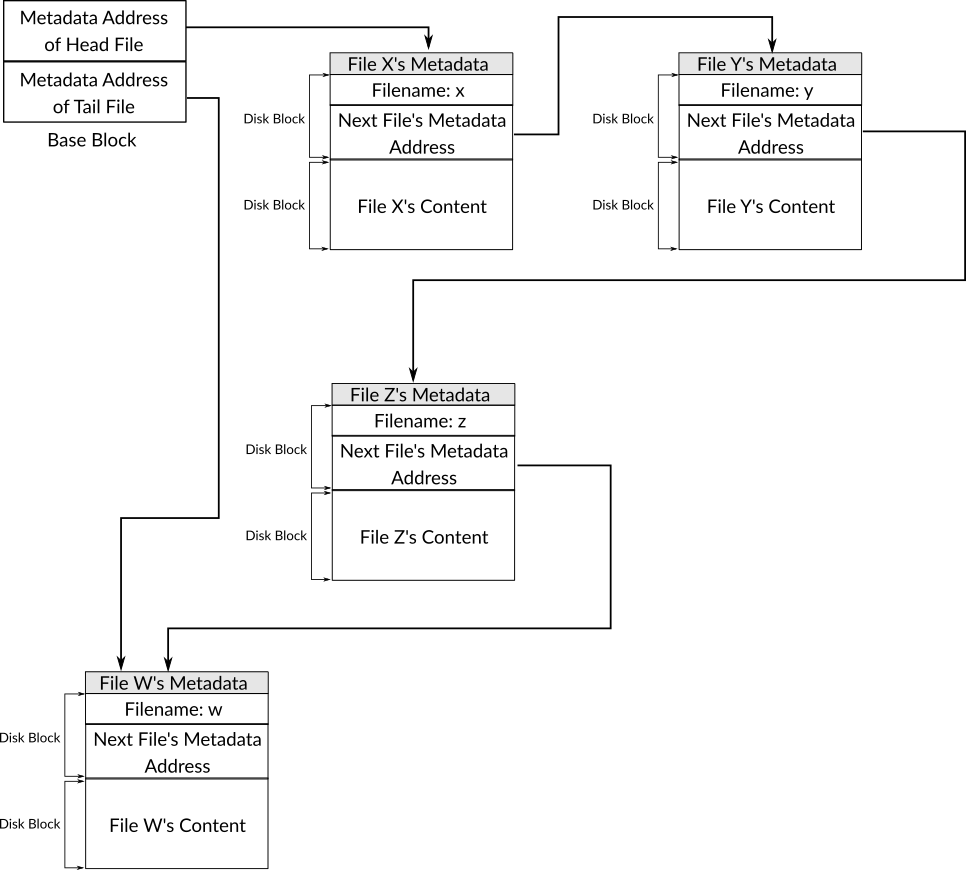
\includegraphics[width=0.75000\textwidth]{Figures/filesystem-ch/539filesystem_overview.png}
\caption{An Overview of 539filesystem
Design}\label{fig:539filesystem_overview}
\end{figure}

In 539filesystem, the block that has the address \lstinline!100! in the
disk is known as the \emph{base block}, from this block we can reach the
whole run-time filesystem. The base block is divided into two parts, the
size of each one of them is \lstinline!4! bytes, the first part is the
address of the metadata of the first file that has been created in the
run-time filesystem, that is, the \emph{head file} \footnote{In
  linked-list data structure's term: the head} while the second part is
the address of the metadata of the last file that has been created in
the run-time filesystem, that is, the \emph{tail file} \footnote{In
  linked-list data structure's term: the tail}.

Each file has its own metadata that contains file's name and the
\emph{next field} which stores the metadata address of the next file
that has been created. The length of the filename is \lstinline!256!
bytes and the size of ``next'' field is \lstinline!4! bytes. When there
is no next file, the value \lstinline!0! is stored in the ``next'' field
of the last file's metadata, that is, the tail file.

It should be obvious now how can we reach all files in a run-time
filesystem that uses 539filesystem, starting from the base block we get
the metadata address of the head file and by using the ``next'' field
from this metadata we can reach the metadata of the next file and the
process continues until we reach the tail file.

The metadata of each file is stored in the block right before the
content of the file which will be stored in one block only given that
the size of a block is \lstinline!512! bytes \footnote{In real-world
  situation, giving a whole block for a metadata of \lstinline!260!
  bytes can be considered as a waste of space. One of real filesystems
  goals is to use as little space as possible to maintain the structure
  of the run-time filesystem.}. For example, if the metadata of file
\lstinline!A! is stored in the address \lstinline!103!, then the content
of this file is stored in the address \lstinline!104!. By using this
design, the basic functionalities of filesystems can be provided. Figure
\ref{fig:539filesystem_overview} shows an overview of 539filesystem
design where four files stored in the system, \lstinline!x!,
\lstinline!y!, \lstinline!z! and \lstinline!w!.

\subsection{The Implementation of
539filesystem}\label{the-implementation-of-539filesystem}

Before getting started in implementing the proposed design in the
previous section, let's define two new files: \lstinline!str.h! and
\lstinline!str.c! which contain string related function that can be
useful when we write our filesystem. Two functions will be implemented
in \lstinline!str.c! and they are \lstinline!strcpy! which copies a
string from a location to another, and \lstinline!strcmp! which compares
two strings, if they are equals then \lstinline!1! is returned,
otherwise \lstinline!0! is returned. There is no need to explain the
details of the code of these two functions since they depend on the
normal way which C uses with strings. The following is the content of
\lstinline!str.h!.

\begin{lstlisting}[language=C]
void strcpy( char *, char * );
int strcmp( char *, char * );
\end{lstlisting}

The following is the content of \lstinline!str.c!.

\begin{lstlisting}[language=C]
#include "str.h"

void strcpy( char *dest, char *src )
{
    int idx = 0;
    
    while ( *src != '\0' )
    {
        dest[ idx ] = *src;
        
        src++;
        idx++;
    }
}

int strcmp( char *str1, char *str2 )
{
    while ( *str1 != '\0' )
    {
        if ( *str1 != *str2 )
            return 0;
        
        str1++;
        str2++;
    }
    
    if ( *str2 != '\0' )
        return 0;
    
    return 1;
}
\end{lstlisting}

Now we can start implementing 539filesystem. The first step as usual is
to create the files that hold the functions related to our filesystem:
\lstinline!filesystem.h! and \lstinline!filesystem.c!. The following is
the content of \lstinline!filesystem.h!.

\begin{lstlisting}[language=C]
#define BASE_BLOCK_ADDRESS 100
#define FILENAME_LENGTH 256

typedef struct
{
    int head, tail;
} base_block_t;

typedef struct
{
    char filename[ FILENAME_LENGTH ];
    int next_file_address;
} metadata_t;

base_block_t *base_block;

void filesystem_init();
void create_file( char *, char * );
char **list_files();
char *read_file( char * );

// Auxiliary Functions
metadata_t *load_metadata( int );
int get_address_by_filename( char * );
int get_prev_file_address( int );
int get_files_number();
\end{lstlisting}

First we define two macros, \lstinline!BASE_BLOCK_ADDRESS! and
\lstinline!FILENAME_LENGTH!. The first one is the address of base block
in the disk, as we have mentioned earlier, this address is
\lstinline!100!. The second one is the maximum length of a filename in
539filesystem, and we mentioned earlier that this length is
\lstinline!256!.

Then we define two structures as types: \lstinline!base_block_t! and
\lstinline!metadata_t!, based on our discussions on 539filesystem
design, you may have noticed that \lstinline!base_block_t! represents
the base block, it has two fields, each one of them of size
\lstinline!4! bytes, the first one is \lstinline!head! and the second
one is \lstinline!tail!. The type \lstinline!metadata_t! represents the
metadata of a file, it has two fields as we described before, the first
one is the filename and the second one is the metadata address of the
next file. These two structures are based on linked-list data structure,
and we are going to use them to load the data that they represent from
the disk, manipulate them while they are in the main memory, then write
them back to the disk in order to make the run-time filesystem
persistent.

Then the global variable \lstinline!base_block! is defined, which is the
memory address that contains the base block after loading it from the
disk, as we have said, this loaded copy is the one that we are going to
update when the user performs a transactional operation on the run-time
filesystem such as creating a new file for example.

After including \lstinline!filesystem.h! in \lstinline!filesystem.c! the
first function that we are going to implement is
\lstinline!filesystem_init! which is an initializer that will be called
once the kernel starts. Its code is too simple, it is going to use the
ATA device driver to read the base block from the disk to the main
memory and stores the memory address of this loaded data in the global
variable \lstinline!base_block!.

\begin{lstlisting}[language=C]
void filesystem_init()
{
    base_block = read_disk( BASE_BLOCK_ADDRESS );
}
\end{lstlisting}

We need to include \lstinline!filesystem.h! in \lstinline!main.c! and
call function \lstinline!filesystem_init! by putting the line
\lstinline!filesystem_init();! in \lstinline!kernel_main! of
\lstinline!main.c! after the line \lstinline!scheduler_init();!. The
rest of functions will be discussed in the following sub-sections.

\subsubsection{Creating a New File}\label{creating-a-new-file}

Let's begin with the function \lstinline!create_file!, we mentioned
before that there is no write operation in 539filesystem, instead, the
content of a new file is written in the same operation that creates a
new file. Basically, \lstinline!create_file! operation should decide the
disk address that the new file and its metadata should be stored in, of
course, in real-world situation, the filesystem should be sure that this
disk address is free and doesn't contain a part of another file. After
deciding the disk address of this new file, the metadata of the file
should be stored in the block that this address points to, and in the
next block the content of this file should be stored. The metadata of
the new file can be initialized by using the type \lstinline!metadata_t!
and after that it can be stored into the disk by using ATA device
driver.

Beside writing the metadata and the content of the file on the disk,
creating a new file in 539filesystem is equivalent to inserting a new
item in a linked-list, so, the base block need to be modified to make
sure that the new file is reachable later. To do that, the metadata
address of the new file should replace the tail in the base block, that
is, the metadata address that was the tail before creating the new file
is not the tail anymore, it become a normal item in the list that was
once the tail and it can be reached via the ``next'' field of the file
before it. The ``next'' field of this previous tail should be updated to
point to the newly created file, and the tail in base block should be
updated in the base block to point to the newly created file. There are
also more subtle cases in updating the base block that will be discussed
while writing the code of \lstinline!create_file!. Let's start with the
first part of the function.

\begin{lstlisting}[language=C]
void create_file( char *filename, char *buffer )
{
    int metadata_lba = ( base_block->head == 0 ) ? BASE_BLOCK_ADDRESS + 1 : base_block->tail + 2;
    int file_lba = metadata_lba + 1;
    
    metadata_t *metadata = kalloc( sizeof( metadata_t ) );
    
    metadata->next_file_address = 0;
    
    int currIdx;
    
    for ( currIdx = 0; *filename != '\0' && currIdx < FILENAME_LENGTH - 1; currIdx++, filename++ )
        metadata->filename[ currIdx ] = *filename;
    
    metadata->filename[ currIdx ] = '\0';
    
    write_disk( metadata_lba, metadata );
    write_disk( file_lba, buffer );
\end{lstlisting}

When the value of the head in the base block is \lstinline!0!, that
means there is no files at all in the run-time filesystem. When
\lstinline!create_file! is called in this situation, that means this
file that the caller is requesting to create is the first file in the
run-time filesystem, the metadata of this first file can be simply
stored in the block right after the base block. In
\lstinline!create_file! this fact is used to decide the disk address for
the metadata of the new file, this address is stored in the local
variable \lstinline!metadata_lba! which its name is a short for
``metadata logical block address''. Figure
\ref{fig:create_file_empty_case} shows the state of 539filesystem after
creating the first file \lstinline!A! in the run-time filesystem.

\begin{figure}
\centering
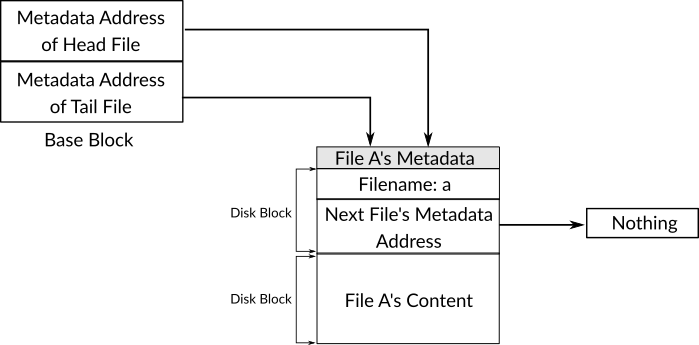
\includegraphics[width=0.65000\textwidth]{Figures/filesystem-ch/create_file_empty_case.png}
\caption{The State 539filesystem After Creating the First
File}\label{fig:create_file_empty_case}
\end{figure}

In case that the run-time filesystem is not empty, that is, the value of
\lstinline!head! is not \lstinline!0!, then the tail field of base block
can be used to decide the metadata address of the new file. As we know,
the tail field contains the metadata address of the last file that has
been added to the run-time filesystem, and the content of that file is
stored in the disk address \lstinline!tail + 1!, which means
\lstinline!tail + 2! is a free block that can be used to store new data
\footnote{This is ensured since 539filesystem stores the files in order,
  so, there will be no files after the tail unless it is a deleted file
  which can be overwritten and causes no data lose.}, so we choose this
address for the new metadata in this case. After that, the disk address
of the new content is decided by simply adding \lstinline!1! to the disk
address of the new metadata, the address of the content is stored in the
local variable \lstinline!file_lba!.

After deciding the disk addresses of the new metadata and file content,
we start in creating the metadata of the file to store them later on the
disk. As you can see in the code, we allocate a space in the kernel's
heap for the new metadata by depending on the type
\lstinline!metadata_t!, after this allocation, we can use the local
variable \lstinline!metadata! to fill the fields of the new file
metadata. First, we set the value of the ``next'' field to
\lstinline!0!, because, as we mentioned earlier, this new file will be
the tail file which means there is no file after it. Then, we copy the
filename which is passed as a parameter \lstinline!filename! to the
filename field of the metadata, in case the passed filename's length is
less than the maximum length, then the whole filename is copied,
otherwise, only the maximum number of characters of the passed filename
is copied and the rest are simply ignored. The final step that is
related to the new file is to write the metadata and the file content in
the right addresses on the disk, and this is done in the last two lines
which use the ATA device driver. The following is the next and last part
of \lstinline!create_file! which updates the base block depending on the
current state of the run-time filesystem.

\begin{lstlisting}[language=C]
    if ( base_block->head == 0 )
    {
        update_base_block( metadata_lba, metadata_lba );
    }
    else
    {   
        metadata_t *tail_metadata = load_metadata( base_block->tail );
        
        tail_metadata->next_file_address = metadata_lba;
        
        write_disk( base_block->tail, tail_metadata );      
        update_base_block( base_block->head, metadata_lba );
    }
} // End of "create_file"
\end{lstlisting}

When the run-time filesystem is empty, that is, the value of
\lstinline!head! in the base block is \lstinline!0!, then the new file
that we are creating will be both the head and the tail file. As you can
see, in the block of \lstinline!if! statement that checks whether
\lstinline!head! equals \lstinline!0! or not, the not defined yet
function \lstinline!update_base_block! is used, this function updates
the values of \lstinline!head! and \lstinline!tail! of the base block
and write these changes on the permanent copy of the base block on the
disk, the disk address of the new file's metadata is simply set as head
and tail when \lstinline!update_base_block! is called in this case.

The second case is when the run-time filesystem isn't empty, that is,
the value of \lstinline!head! isn't \lstinline!0!. In this case we need
to update the disk address of the tail in the base block to consider the
new file as the new tail, furthermore, the ``next'' field of the
previous tail, which is not the tail anymore, should be updated to point
to the metadata of the new file, you see in \lstinline!else! block that
this is exactly what is done.

The function that isn't defined yet \lstinline!load_metadata! is used to
load the metadata of the previous tail by passing the its disk address a
parameter. After that, the local variable \lstinline!tail_metadata! will
point to that loaded metadata of the tail, and depending on the type
\lstinline!metadata_t! we can reach the values of the previous tail
fields easily. You can see that we simply changed the value of the
``next'' field to the metadata address of the new file, then we write
this modification on the disk and of course on the same location,
finally, the tail field is updated in the base block by calling
\lstinline!update_base_block! which its code is presented next. Figure
\ref{fig:create_file_not_empty_case} shows the steps needed to create a
new file in 539filesystem as described and implemented in the function
\lstinline!create_file!.

\begin{lstlisting}[language=C]
void update_base_block( int new_head, int new_tail )
{
    base_block->head = new_head;
    base_block->tail = new_tail;
    
    write_disk( BASE_BLOCK_ADDRESS, base_block );
}
\end{lstlisting}

It's too simple, it receives the value of head and tail that we would
like to set on the base block, then, the copy of the base block which is
stored in the main memory is updated, then, this updated version is
overwritten on the base block address on the disk. The following is code
of \lstinline!load_metadata! which has been used in
\lstinline!create_file! function.

\begin{figure}
\centering
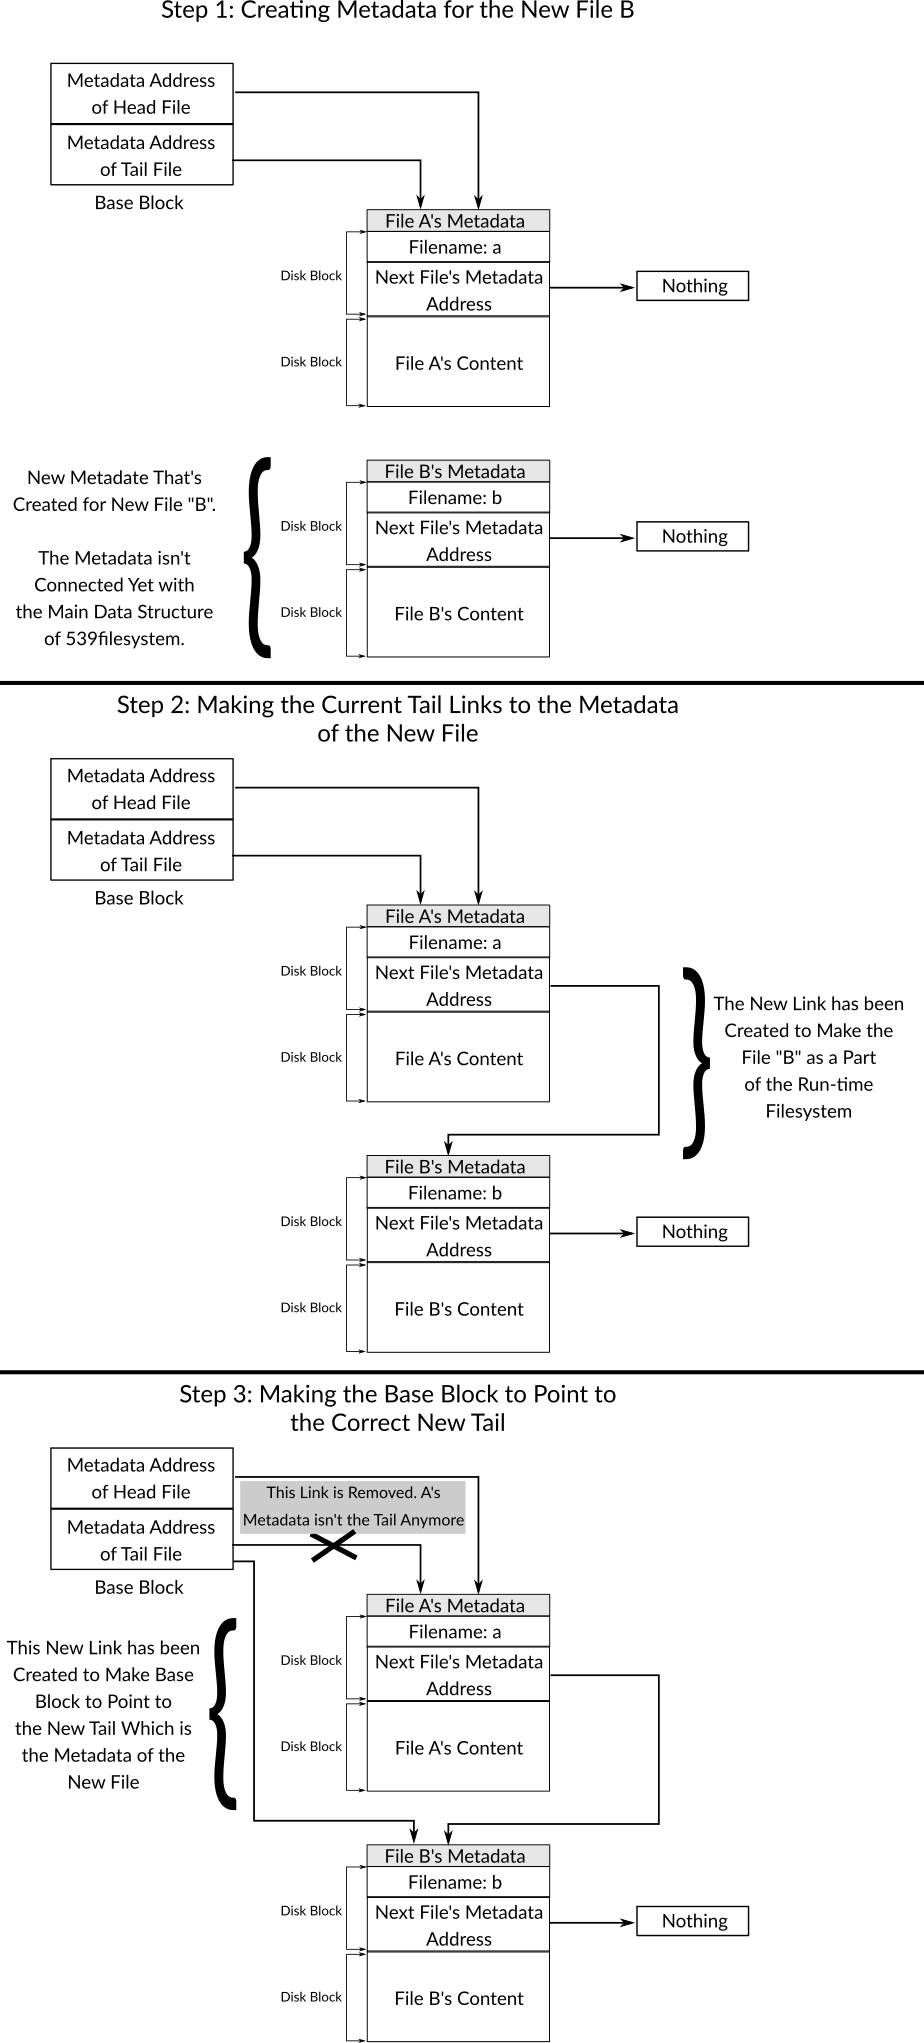
\includegraphics[width=0.85000\textwidth]{Figures/filesystem-ch/create_file_not_empty_case.png}
\caption{Steps Needed to Create New File in 539filesystem When Run-time
Filesystem isn't Empty}\label{fig:create_file_not_empty_case}
\end{figure}

\begin{lstlisting}[language=C]
metadata_t *load_metadata( int address )
{
    metadata_t *metadata = read_disk( address );
    
    return metadata;
}
\end{lstlisting}

Simply, it receives a disk address and assumes that the block which is
presented by this address is a metadata block. It loads this metadata to
the main memory by loading the content of the address from the disk
through the device driver function \lstinline!read_disk!. The following
is a sample of using \lstinline!create_file! to create a new file in the
run-time filesystem.

\begin{lstlisting}[language=C]
char *data = kalloc( 512 );

strcpy( data, "The content of the first file on 539filesystem" );
    
create_file( "first_file", data );
\end{lstlisting}

\subsubsection{Listing All Files}\label{listing-all-files}

To list all files on 539filesystem, the normal traversal algorithm of
linked-list can be used. In linked-list, to traverse all list's item you
need to start with the head of the list, then to reach the second item
of the list, the ``next'' field of the head can be used, and so on for
the rest of items in the linked-list. The ``next'' field is the
component which links the items of the list with each other. You keep
traversing the items until the tail of the list is reached and you can
check whether the current item is the tail or not by checking its
``next'' field, in case its value is \lstinline!0! (or usually in
higher-level implementations \lstinline!NULL!) then you know that the
current item is the tail which means the list is over. Another way to
check if the current item is the tail is by comparing its address with
the one which is stored in the tail field of the linked-list, in our
case, the base block. The following is the code of the function
\lstinline!list_files! which uses the algorithm we just described, it
returns an array of strings, each item of this array is a filename.

\begin{lstlisting}[language=C]
char **list_files()
{
    // Part 1
    
    if ( base_block->head == 0 )
        return -1;
    
    // Part 2
    
    char **list;
    
    list = kalloc( get_files_number() * sizeof( char * ) );
    
    // Part 3
    
    metadata_t *curr_file = load_metadata( base_block->head );
    
    int idx = 0;
    
    while ( 1 )
    {
        list[ idx ] = curr_file->filename;

        if ( curr_file->next_file_address == 0 )
            break;
        
        curr_file = load_metadata( curr_file->next_file_address );
        
        idx++;
    }
    
    return list;
}
\end{lstlisting}

The first part of \lstinline!list_files! handles the case where the
run-time filesystem is empty, so, it returns \lstinline!-1! to indicate
that there is no files to list. In case that the run-time filesystem
isn't empty, the function in the second part allocates a space in
kernel's heap for the list of the filenames, as you can see, we have
used a function named \lstinline!get_files_number! to decide how many
bytes we are going to allocate for this list, based on its name, this
function returns the number of files in the run-time filesystem, its
code will be presented in a moment. In the third part, the function is
ready to traverse the list of files metadata which are stored in the
disk and are reachable starting from the disk address which is stored in
the head field in the base block.

Initially, the metadata of the head file is loaded into memory and can
be accessed through the local variable \lstinline!curr_file!, then, the
loop is started. In the body of the loop, the filename of the current
file metadata is appended to the result's variable \lstinline!list!, in
the first iteration of this loop the filename will be the one that
belong to the head file. After appending the filename of the current
file to \lstinline!list!, the function checks if the current file is the
tail file or not by checking the value of the ``next'' field
\lstinline!next_file_address!, if it is \lstinline!0! then the current
file is the tail, so, the loop should break and the result should be
returned to the caller. In case that the current file isn't the tail
file, then the metadata of the next file is loaded by using the disk
address which is stored in the ``next'' field of the current file, the
current value of \lstinline!curr_file! is replaced with a memory address
that points to the metadata of the next file which will be used in the
next iteration of the loop, the same operation continues until the
function reaches the tail which breaks the loop and returns the list to
the caller. The following is the code of \lstinline!get_files_number!
that was used in \lstinline!list_files! and, as mentioned earlier,
returns the number of stored files.

\begin{lstlisting}[language=C]
int get_files_number()
{
    if ( base_block->head == 0 )
        return 0;
    
    int files_number = 0;
    
    // ... //
    
    metadata_t *curr_file = load_metadata( base_block->head );
    
    while ( 1 )
    {
        files_number++;

        if ( curr_file->next_file_address == 0 )
            break;
        
        curr_file = load_metadata( curr_file->next_file_address );
    }
    
    return files_number;
}
\end{lstlisting}

As you can see, it works in a similar way as \lstinline!list_files!, the
main difference is that \lstinline!get_files_number! keep tracking the
number of iterations to fetch the number of files instead of copying the
filename of the current file to another list. The following is a sample
of using \lstinline!list_files!.

\begin{lstlisting}[language=C]
void print_fs()
{
    char **files = list_files();

    for ( int currIdx = 0; currIdx < get_files_number(); currIdx++ )
    {
        print( "File: " );
        print( files[ currIdx ] );
        println();
    }
    
    print( "==" );
    println();
}
\end{lstlisting}

\subsubsection{Reading a File}\label{reading-a-file}

The function \lstinline!read_file! reads the content of a file which its
name is passed as a parameter, then, the address of the buffer that
stores that content of the file is returned to the caller. Because the
file size in 539filesystem is always \lstinline!512! bytes then
\lstinline!read_disk! of ATA device driver can be called just one time
to load a file.

To implement \lstinline!read_file!, the main thing to do is to find the
disk address of the file that the caller passed its name as a parameter,
after knowing how to traverse the list of files in 539filesystem, we can
easily use this algorithm to find the disk address of a file given its
name. The following is the code of \lstinline!read_file!.

\begin{lstlisting}[language=C]
char *read_file( char *filename )
{
    int address = get_address_by_filename( filename );
    
    if ( address == 0 )
        return 0;

    char *buffer = read_disk( address + 1 );
    
    return buffer;
}
\end{lstlisting}

The task of finding the disk address of the file's metadata is performed
by the function \lstinline!get_address_by_filename! which we will define
in a moment. When the metadata of the file is not found,
\lstinline!read_file! returns \lstinline!0!, otherwise, the file will be
read by calling \lstinline!read_disk!, as you can see, the parameter
that is passed to this function is \lstinline!address + 1! since the
value of \lstinline!address! is the disk address of the file's metadata
and not its content. Finally, the address of the buffer is returned to
the caller. The following is the code of
\lstinline!get_address_by_filename!.

\begin{lstlisting}[language=C]
int get_address_by_filename( char *filename )
{
    metadata_t *curr_file = load_metadata( base_block->head );
    int curr_file_address = base_block->head;
    
    int idx = 0;
    
    while ( 1 )
    {
        if ( strcmp( curr_file->filename, filename ) == 1 )
            return curr_file_address;
            
        if ( curr_file->next_file_address == 0 )
            break;
        
        curr_file_address = curr_file->next_file_address;
        curr_file = load_metadata( curr_file->next_file_address );      
    }
    
    return 0;
}
\end{lstlisting}

This function receives a filename as a parameter, then, it traverse the
list of the files, with each iteration, the name of the current file is
compared to the passed filename by using the function \lstinline!strcmp!
that we already defined, if the name of the current file doesn't match
the passed filename, the function loads the metadata of the next file by
using \lstinline!load_metadata! and continues to the next iteration of
the loop to check whether the next file is the required file or not, and
so on, if the file isn't found, then the loop exits and \lstinline!0! is
returned. When a match is found, the disk address of the current file's
metadata which is stored in the local variable
\lstinline!curr_file_address! is returned to the caller. The following
is a sample of using \lstinline!read_file!.

\begin{lstlisting}[language=C]
print( read_file( "first_file" ) );
\end{lstlisting}

\subsubsection{Deleting a File}\label{deleting-a-file}

As in creating a file, deleting a file may cause modifications on the
base block or even on another file's metadata. Given a filename, the
function \lstinline!delete_file! deletes this file from the run-time
filesystem, technically, the content of the file will not be overwritten
with zeros for example, instead, only the reference to this file is
removed from either the base block in case that file is the head, from
another file's ``next'' field or both in case that is file is the tail.

As mentioned earlier, this design decision of not overwriting the
content of the file, that the user would like to delete, with zeros for
example on the disk is taken in real-world filesystems to make the
delete process faster and this decision made it possible for deleted
files recovery software to exist, this type of software can recover
deleted files since their contents are still on the disk but there is
not reference to them in the run-time filesystem's data structure,
however, the space of deleted files are considered as free space by the
filesystem and it can be used anytime, that's why the recovery software
cannot ensure you that it could recover all deleted files because the
space which was occupied by the deleted file (or part of it) may be now
used by another file. The following is the code of
\lstinline!delete_file!.

\begin{lstlisting}[language=C]
void delete_file( char *filename )
{   
    // Part 1
    
    int curr_file_address = get_address_by_filename( filename );
    
    if ( curr_file_address == 0 )
        return;
    
    metadata_t *curr_file_metadata = read_disk( curr_file_address );
    
    // Part 2
    
    if ( get_files_number() == 1 )
    {
        update_base_block( 0, 0 );
        
        return;
    }
    
    // Part 3
    if ( curr_file_address == base_block->head )
    {
        update_base_block( curr_file_metadata->next_file_address, base_block->tail );
    }
    // Part 4
    else
    {
        int prev_file_address = get_prev_file_address( curr_file_address );
        
        metadata_t *prev_file = load_metadata( prev_file_address );

        prev_file->next_file_address = curr_file_metadata->next_file_address;
        
        write_disk( prev_file_address, prev_file );
        
        if ( curr_file_address == base_block->tail )
            update_base_block( base_block->head, prev_file_address );
    }
}
\end{lstlisting}

The first part tries to find the metadata address of the file in
question by using the function \lstinline!get_address_by_filename!, in
case the file is not found, the function does nothing and returns.
Otherwise, the metadata of the file is loaded and the local variable
\lstinline!curr_file_metadata! is used to point to that metadata in the
main memory.

In the second part, the most basic case of deleting a file is handled,
when there is only one file in the run-time filesystem, nothing need to
be done but updating the base block to indicate that the disk address of
both head and tail is \lstinline!0! which means, as mentioned earlier,
that the run-time filesystem is empty. The function
\lstinline!update_base_block! is used to update the base block. Figure
\ref{fig:delete_file_one_file_case} shows this case.

\begin{figure}
\centering
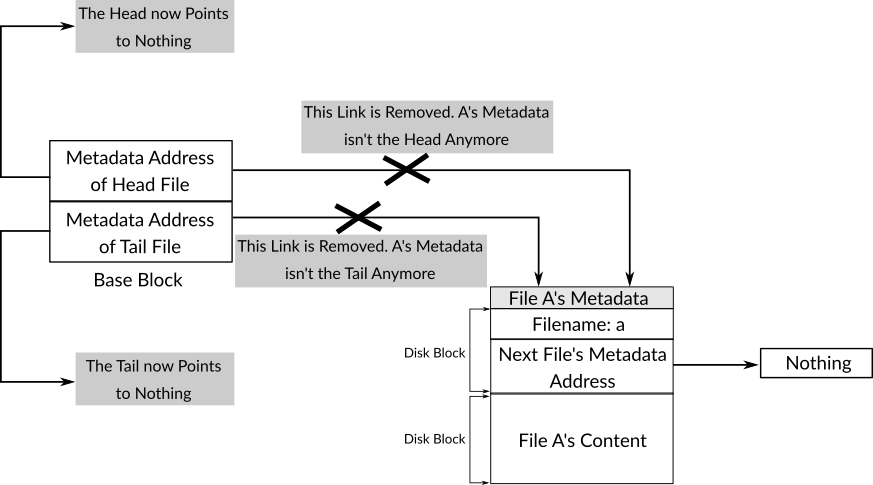
\includegraphics[width=0.80000\textwidth]{Figures/filesystem-ch/delete_file_one_file_case.png}
\caption{The State 539filesystem After Removing the Only
File}\label{fig:delete_file_one_file_case}
\end{figure}

The third part handles the case where the file to be deleted is the head
file, in this case, to remove the reference of this file, we simply
replace the current value of the \lstinline!head! in base block with the
metadata address of the file right next to the head which can be found
in the ``next'' field of the current head, so, the second file will
become the head file after finishing the delete process. Figure
\ref{fig:delete_file_head_case} shows this case.

\begin{figure}
\centering
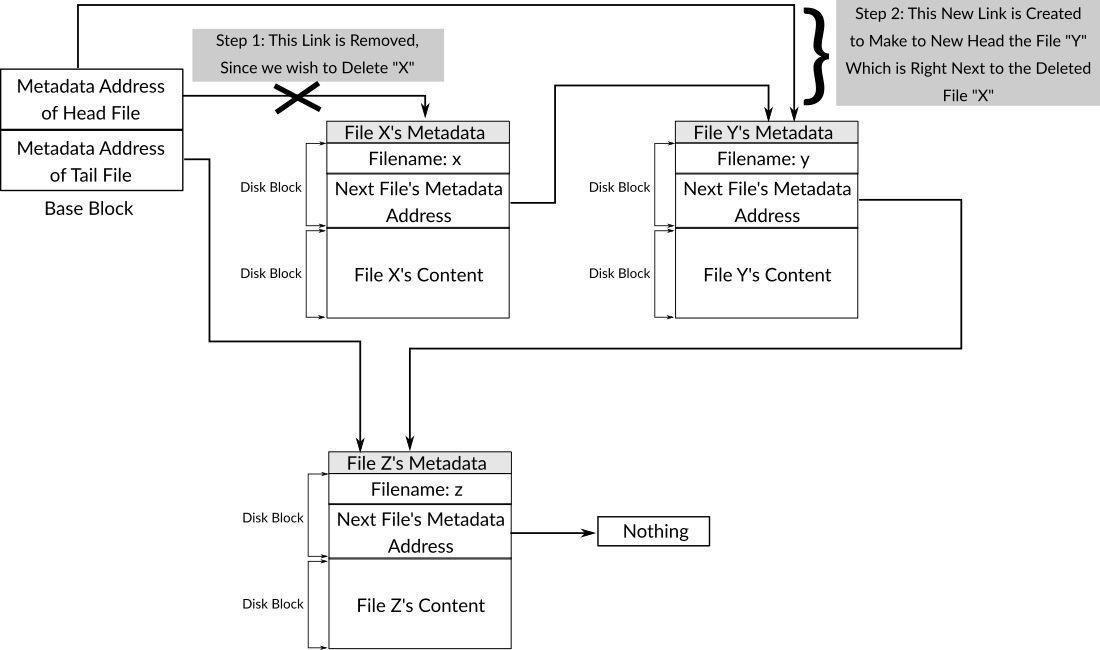
\includegraphics[width=1.00000\textwidth]{Figures/filesystem-ch/delete_file_head_case.png}
\caption{The Steps Needed to Delete the Head File in
539filesystem}\label{fig:delete_file_head_case}
\end{figure}

The fourth part of the function handles the case where the file to be
deleted is not the head, in this case, the previous file's metadata
needs to be found to modify its ``next'' field by replacing it with the
value of the ``next'' field of the file that we would like to delete, in
this way, we will be sure that the reference of the file to be deleted
is removed from 539filesystem data structure, and that the previous file
is linked with the next file. Figure \ref{fig:delete_file_not_head_case}
shows this case. Also, in this case, the file in question may be the
tail, therefore, the tail on the base block should be replaced with the
disk address of the previous file's metadata. Figure
\ref{fig:delete_file_not_head_but_tail_case} shows this case.

\begin{figure}
\centering
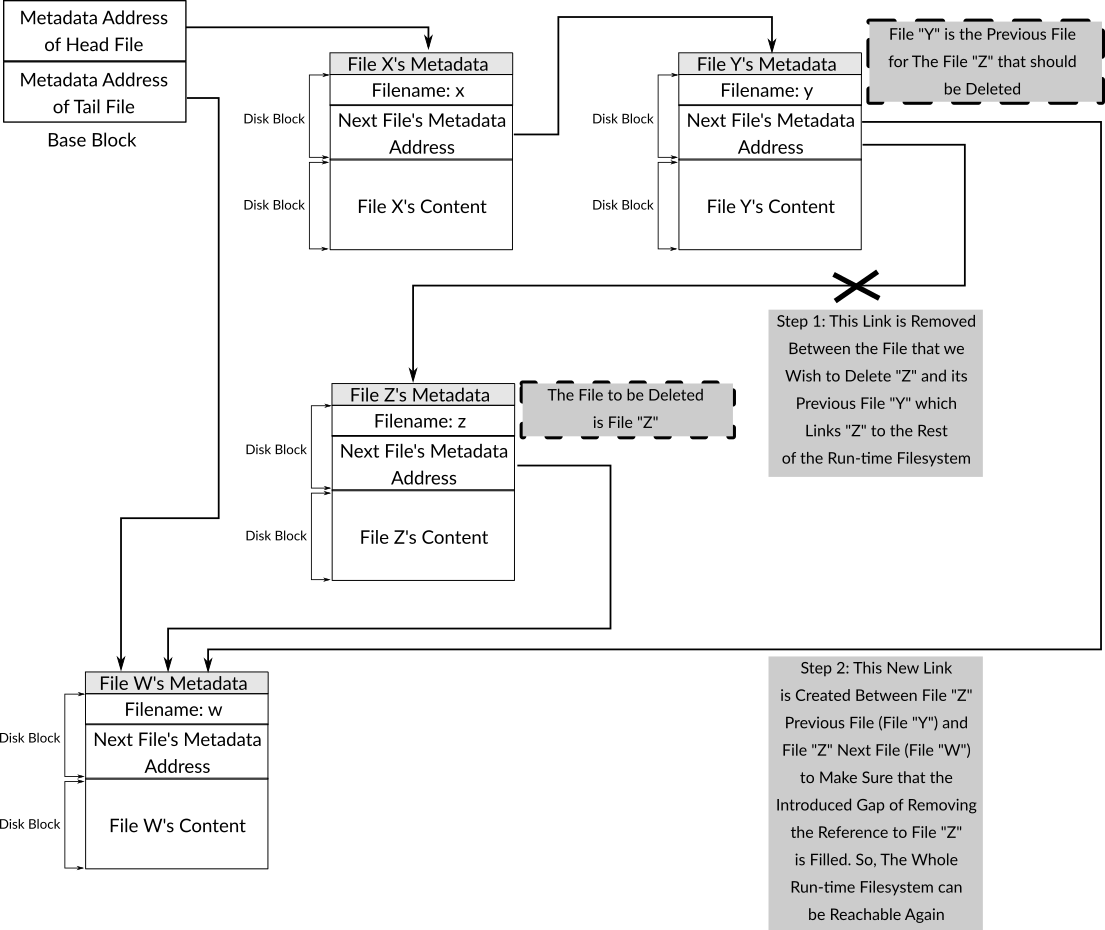
\includegraphics[width=1.00000\textwidth]{Figures/filesystem-ch/delete_file_not_head_case.png}
\caption{The Steps Needed to Delete a File which is not the
Head}\label{fig:delete_file_not_head_case}
\end{figure}

\begin{figure}
\centering
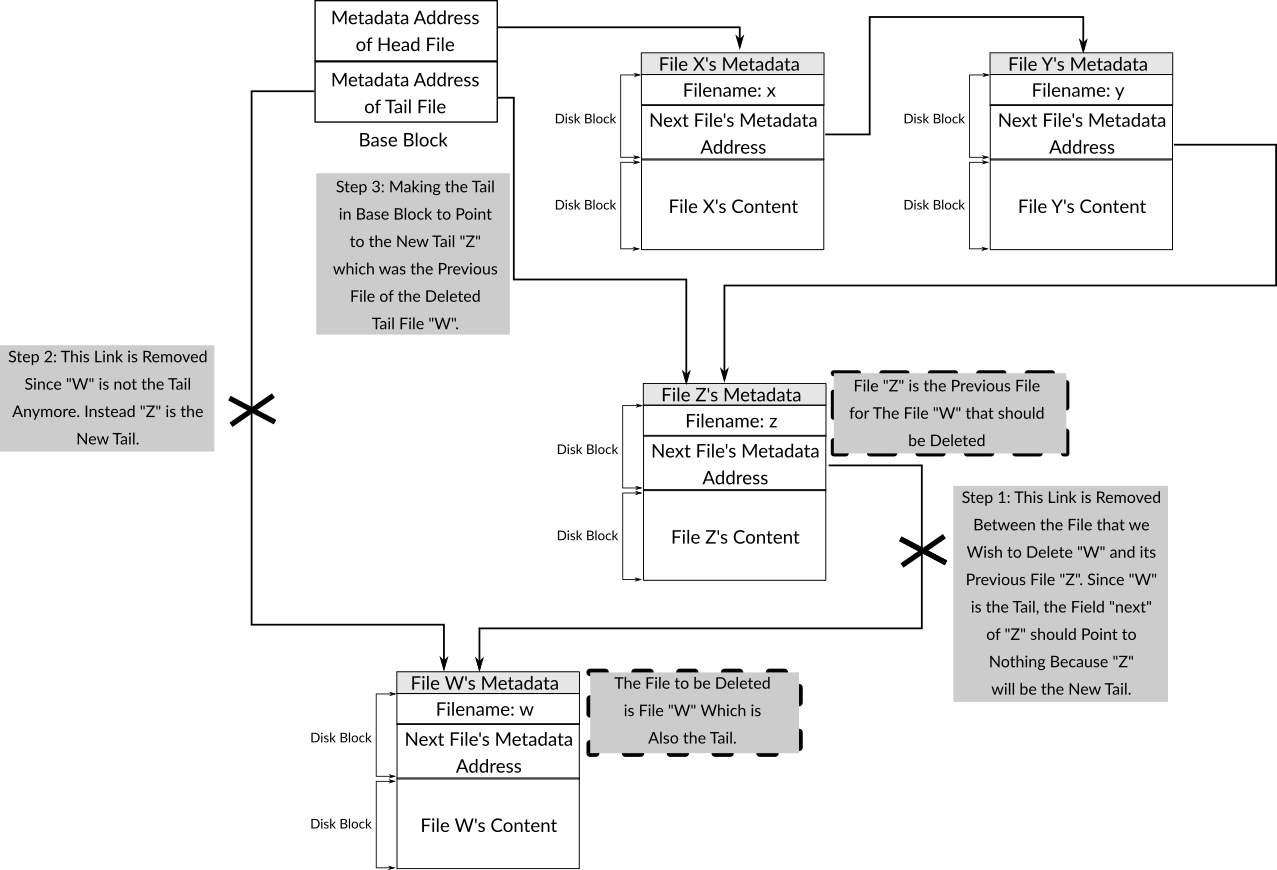
\includegraphics[width=1.00000\textwidth]{Figures/filesystem-ch/delete_file_not_head_but_tail_case.png}
\caption{The Steps Needed to Delete a File which is not the Head but
it's a Tail in 539filesystem. The File to Delete Here is
``W''.}\label{fig:delete_file_not_head_but_tail_case}
\end{figure}

As you can see in the first code line of this fourth part, a function
named \lstinline!get_prev_file_address! is used to get the disk address
of previous file's metadata to be able to perform the described
operation. By using this address, the metadata is loaded by using
\lstinline!load_metadata! in order to modify the ``next'' field of the
previous file, the updated metadata is written on the same address in
the disk. Finally, the function checks if the file to be deleted is the
tail file or not, if this is the case, the tail in base block is updated
to point to the previous file which ensures that there is no any
reference to that file in the filesystem's data structure. The following
is the code of \lstinline!get_prev_file_address! which needs no more
explanation.

\begin{lstlisting}[language=C]
int get_prev_file_address( int address )
{
    metadata_t *prev_file = load_metadata( base_block->head );
    int prev_file_address = base_block->head;

    while ( 1 )
    {
        if ( prev_file->next_file_address == address )
            return prev_file_address;
        
        prev_file_address = prev_file->next_file_address;
        prev_file = load_metadata( prev_file->next_file_address );
    }
        
    return -1;
}
\end{lstlisting}

\section{\texorpdfstring{Finishing up Version \texttt{NE} and Testing
the
Filesystem}{Finishing up Version NE and Testing the Filesystem}}\label{finishing-up-version-ne-and-testing-the-filesystem}

And now version \lstinline!NE! of 539kernel is ready. It contains a
basic ATA device driver and 539filesystem. The following is its
\lstinline!Makefile! which adds the new files to the compilation list,
also, this time we are going to use Bochs instead of QEMU to test
539filesystem since \lstinline!kernel.img! which represents the hardisk
is tailored for the former.

\begin{lstlisting}[language=make]
ASM = nasm
CC = gcc
BOOTSTRAP_FILE = bootstrap.asm 
SIMPLE_KERNEL = simple_kernel.asm
INIT_KERNEL_FILES = starter.asm
KERNEL_FILES = main.c
KERNEL_FLAGS = -Wall -m32 -c -ffreestanding -fno-asynchronous-unwind-tables -fno-pie
KERNEL_OBJECT = -o kernel.elf

build: $(BOOTSTRAP_FILE) $(KERNEL_FILE)
    $(ASM) -f bin $(BOOTSTRAP_FILE) -o bootstrap.o
    $(ASM) -f elf32 $(INIT_KERNEL_FILES) -o starter.o 
    $(CC) $(KERNEL_FLAGS) $(KERNEL_FILES) $(KERNEL_OBJECT)
    $(CC) $(KERNEL_FLAGS) screen.c -o screen.elf
    $(CC) $(KERNEL_FLAGS) process.c -o process.elf
    $(CC) $(KERNEL_FLAGS) scheduler.c -o scheduler.elf
    $(CC) $(KERNEL_FLAGS) heap.c -o heap.elf
    $(CC) $(KERNEL_FLAGS) paging.c -o paging.elf
    $(CC) $(KERNEL_FLAGS) ata.c -o ata.elf
    $(CC) $(KERNEL_FLAGS) str.c -o str.elf
    $(CC) $(KERNEL_FLAGS) filesystem.c -o filesystem.elf
    ld -melf_i386 -Tlinker.ld starter.o kernel.elf screen.elf process.elf scheduler.elf heap.elf paging.elf ata.elf str.elf filesystem.elf -o 539kernel.elf
    objcopy -O binary 539kernel.elf 539kernel.bin
    dd if=bootstrap.o of=kernel.img
    dd seek=1 conv=sync if=539kernel.bin of=kernel.img bs=512 count=20
    dd seek=21 conv=sync if=/dev/zero of=kernel.img bs=512 count=2046
    bochs -f bochs
\end{lstlisting}

To run Bochs, it should be configured properly. As you can see from the
presented \lstinline!Makefile!, a file named \lstinline!bochs! is passed
to Bochs to use it as a configuration file, so, by using it we don't
need to configure Bochs everytime we use it to run 539kernel. The
following is the content of \lstinline!bochs! file which should reside
in the same directory of 539kernel's code.

\begin{lstlisting}
plugin_ctrl: unmapped=1, biosdev=1, speaker=1, extfpuirq=1, parallel=1, serial=1, gameport=1, iodebug=1
config_interface: textconfig
display_library: x, options="gui_debug"
memory: host=32, guest=32
romimage: file="/usr/share/bochs/BIOS-bochs-latest"
vgaromimage: file="/usr/share/bochs/VGABIOS-lgpl-latest"
boot: disk
ata0: enabled=1, ioaddr1=0x1f0, ioaddr2=0x3f0, irq=14
ata0-master: type=disk, mode=flat, translation=auto, path="kernel.img", cylinders=2, heads=16, spt=63, biosdetect=auto, model="Generic 1234"
pci: enabled=1, chipset=i440fx
vga: extension=vbe, update_freq=5
cpu: count=1, ips=4000000, model=bx_generic, reset_on_triple_fault=1, cpuid_limit_winnt=0, ignore_bad_msrs=1, mwait_is_nop=0
cpuid: family=6, model=0x03, stepping=3, mmx=1, apic=xapic, sse=sse2, sse4a=0, sep=1, aes=0, xsave=0, xsaveopt=0, movbe=0, adx=0, smep=0, avx=0, avx_f16c=0, avx_fma=0, bmi=0, xop=0, tbm=0, fma4=0, vmx=1, x86_64=1, 1g_pages=0, pcid=0, fsgsbase=0, mwait=1
cpuid: vendor_string="GenuineIntel"
cpuid: brand_string="              Intel(R) Pentium(R) 4 CPU        "
\end{lstlisting}

As you can see, it tells Bochs the specifications of the virtual machine
we would like to run, also, the file which represents the hard disk
\lstinline!kernel.img! is passed to Bochs here. The following code can
be used to test 539filesystem. It should be inside
\lstinline!kernel_main! after the initializations and processes
creations.

\begin{lstlisting}[language=C]
    char *data = kalloc( 512 );
    strcpy( data, "The content of the first file on 539filesystem" );   
    create_file( "first_file", data );
    
    // ... //
    
    char *data2 = kalloc( 512 );
    strcpy( data2, "SECOND FILE in 539filesystem" );
    create_file( "second_file", data2 );
    
    // ... //
    
    char *data3 = kalloc( 512 );
    strcpy( data3, "THIRD FILE in 539filesystem" );
    create_file( "third_file", data3 );
        
    // ... //
    
    print( read_file( "first_file" ) ); println();
    print( read_file( "second_file" ) ); println();
    print( read_file( "third_file" ) ); println();
    
    // ... //
    
    print_fs();
    delete_file( "first_file" );
    print_fs();
\end{lstlisting}

This code creates three files, prints their contents, prints the
run-time filesystem tree through the function \lstinline!print_fs! and
finally deletes the file \lstinline!first_file! then prints the run-time
filesystem tree again to show that the file has been deleted
successfully. The function \lstinline!print_fs! already defined in this
chapter. To make everything works file, you need to keep the definition
of \lstinline!print_fs! below \lstinline!kernel_main! and put the
prototype \lstinline!void print_fs();! above \lstinline!kernel_main!.
Also, to test the filesystem you need to make sure that the interrupts
are disabled, the easiest way to do that is modifying
\lstinline!starter.asm! by commenting the line \lstinline!sti! which is
before \lstinline!call kernel_main! in the routine
\lstinline!start_kernel!. After that you should see the result of the
above testing code after the kernel boots up.
